
%%%%%%%%%%%%%%%%%%%%%%%%%%%%%%%%%%%%%%%%%%%%%%%%%%%%%%%%%%%%
%%%%%%%%%%%%%%%%%%%%%%% preamble %%%%%%%%%%%%%%%%%%%%%%%%%%%
%%%%%%%%%%%%%%%%%%%%%%%%%%%%%%%%%%%%%%%%%%%%%%%%%%%%%%%%%%%%

\documentclass[10pt,letterpaper]{article}

\usepackage{opex3}
\usepackage{times}
\usepackage{graphicx}
\graphicspath{{./images/}}
\usepackage{epstopdf}
\usepackage{amsmath}
\usepackage{amssymb}
\usepackage{url}
\usepackage{bm}
\usepackage{enumerate}
\usepackage[]{todonotes} % Add option [disable] to hide all todo notes.
\usepackage{xfrac}
\usepackage{paralist}

%\usepackage{ae} %%for Computer Modern fonts

\usepackage{hyperref}
\hypersetup{pdfborder={0 0 0}}

%
% subfiles is useful for having the abstract (and possible other
% sections/chapters) as separate files.
%
\usepackage{subfiles}

\usepackage[]{siunitx}

%
% The cleveref package seems very cool but currently it doesn't support hebrew
% (babel) very well, so I just use if for single references.
% As a work around I redefine the number definition as suggested in:
% http://tex.stackexchange.com/questions/118235/using-the-cleveref-package-with-hebrew-and-babel
%
\usepackage[capitalise]{cleveref}
\makeatletter
\def\@@number#1{#1}
\makeatother

%
% Some new commands I use in this text
%
\newcommand{\OpSphere}{\bm{\mathcal{S}}}
\newcommand{\OpRot}{\bm{\mathcal{R}}}
\newcommand{\OpDistance}{\bm{\mathcal{D}}}
\newcommand{\OpCumsum}{\bm{\mathcal{C}}}
\newcommand{\OpInt}{\bm{\mathcal{I}}}
\newcommand{\OpCamera}{\bm{\mathcal{P}}}
\newcommand{\Mask}{\bm{M}}
\newcommand{\OpDiag}[1]{\mathrm{diag}\left\{#1\right\}}
\newcommand{\Grad}[1]{\bm{\triangledown_{#1}}}
\newcommand{\argmin}{\mathrm{arg}\min}
\newcommand{\curly}[1]{\left\{#1\right\}}
\newcommand{\roundy}[1]{\left(#1\right)}
\newcommand{\recty}[1]{\left[#1\right]}
\newcommand{\PartDeriv}[2]{\frac{\partial{#1}}{\partial{#2}}}
\newcommand{\vect}[1]{\bm{#1}}
\newcommand{\mat}[1]{\bm{#1}}
\newcommand{\transpose}[1]{{#1}^\intercal}
\newcommand{\derivsym}[1]{\,d{#1}}
\newcommand{\yoavcomment}[1]{}
\renewcommand{\yoavcomment}[1]{#1} % Comment to remove images

\newcommand\authnote[1]{\textsuperscript{\normalfont#1}}
\newcommand\affilnote[1]{\textsuperscript{\normalfont#1}}
\providecommand\textsuperscript[1]{$^{#1}$}

%%%%%%%%%%%%%%%%%%%%%%%%%%%%%%%%%%%%%%%%%%%%%%%%%%%%%%%%%%%%
%%%%%%%%%%%%%%%%%%%%%%% begin %%%%%%%%%%%%%%%%%%%%%%%%%%%%%%
%%%%%%%%%%%%%%%%%%%%%%%%%%%%%%%%%%%%%%%%%%%%%%%%%%%%%%%%%%%%

\begin{document}

%%%%%%%%%%%%%%%%%%%%%%%%%%%%%%%%%%%%%%%%%%%%%%%%%%%%%%%%%%%%
%%%%%%%%%%%%%%%%%% title page information %%%%%%%%%%%%%%%%%%
%%%%%%%%%%%%%%%%%%%%%%%%%%%%%%%%%%%%%%%%%%%%%%%%%%%%%%%%%%%%

\title{Sky Tomography for 3D Aerosol Distribution Recovery}

\author{Amit~Aides,\authnote{1*} Yoav~Y.~Schechner,\authnote{1}
  Vadim~Holodovsky\authnote{1} and Michael~J.~Garay\authnote{2}}

\address{\affilnote{1}Electrical Engineering Department, Technion - Israel Institute of Technology, Haifa 32000, Israel\\
  \affilnote{2}Jet Propulsion Laboratory, California Institute of
  Technology, Pasadena, CA 91109, USA}

\email{\authnote{*}amitibo@tx.technion.ac.il} %% email address is required

% \homepage{http:...} %% author's URL, if desired

%%%%%%%%%%%%%%%%%%%%%%%%%%%%%%%%%%%%%%%%%%%%%%%%%%%%%%%%%%%%
%%%%%%%%%%%%%%%%%%% abstract and OCIS codes %%%%%%%%%%%%%%%%
%%%%%%%%%%%%%%%%%%%%%%%%%%%%%%%%%%%%%%%%%%%%%%%%%%%%%%%%%%%%

%% [use \begin{abstract*}...\end{abstract*} if exempt from copyright]

\begin{abstract}
  Aerosols effect climate, health and aviation.  Currently, their
  retrieval assumes a plane-parallel atmosphere and solely vertical
  radiative transfer (RT). We propose a principle to recover the atmosphere
  as it really is: a three dimensional (3D), volumetric, transparent
  huge object. Tomography is the key to recovery. The process involves
  acquiring the sky lightfield by multi-view wide-angle photography on
  a very large scale. The tomography model is distinct, as the light
  source is unidirectional and uncontrolled, while off-axis scattering
  dominates the images.  We formulate an image formation model based
  on 3D RT. Model inversion is done using optimization
  methods, exploiting a closed-form gradient which we derive for the
  model-fit cost function. The problem is complex but tractable and
  parallelizable, eventually estimating the 3D aerosol distribution.
\end{abstract}

\ocis{(000.0000)
  General.} % REPLACE WITH CORRECT OCIS CODES FOR YOUR ARTICLE

%%%%%%%%%%%%%%%%%%%%%%%%%%%%%%%%%%%%%%%%%%%%%%%%%%%%%%%%%%%%
%%%%%%%%%%%%%%%%%%%%%%% References %%%%%%%%%%%%%%%%%%%%%%%%%
%%%%%%%%%%%%%%%%%%%%%%%%%%%%%%%%%%%%%%%%%%%%%%%%%%%%%%%%%%%%

\bibliography{article}{} \bibliographystyle{osajnl}

%%%%%%%%%%%%%%%%%%%%%%%%%%%%%%%%%%%%%%%%%%%%%%%%%%%%%%%%%%%%
%%%%%%%%%%%%%%%%%%%%%%%%%% body %%%%%%%%%%%%%%%%%%%%%%%%%%
%%%%%%%%%%%%%%%%%%%%%%%%%%%%%%%%%%%%%%%%%%%%%%%%%%%%%%%%%%%%

\section{Introduction}
\label{sec:intro}

Lightfield and integral imaging~\cite{bishop,horstmeyer,kim,Ng1948}
samples the optical radiance distribution in location and
direction. It is mainly used in small-scale setups. This paper deals
with a huge scale, up to Earth's size.  The atmosphere allows light to
pass through in multiple locations and directions. Light is affected
by this medium. Therefore, in this paper we lay out a principle to
recover this 3D medium using measured and modeled lightfields
(Fig.~\ref{fig:groundgrid}).
\begin{figure*}[t!]
  \begin{center}
    \yoavcomment{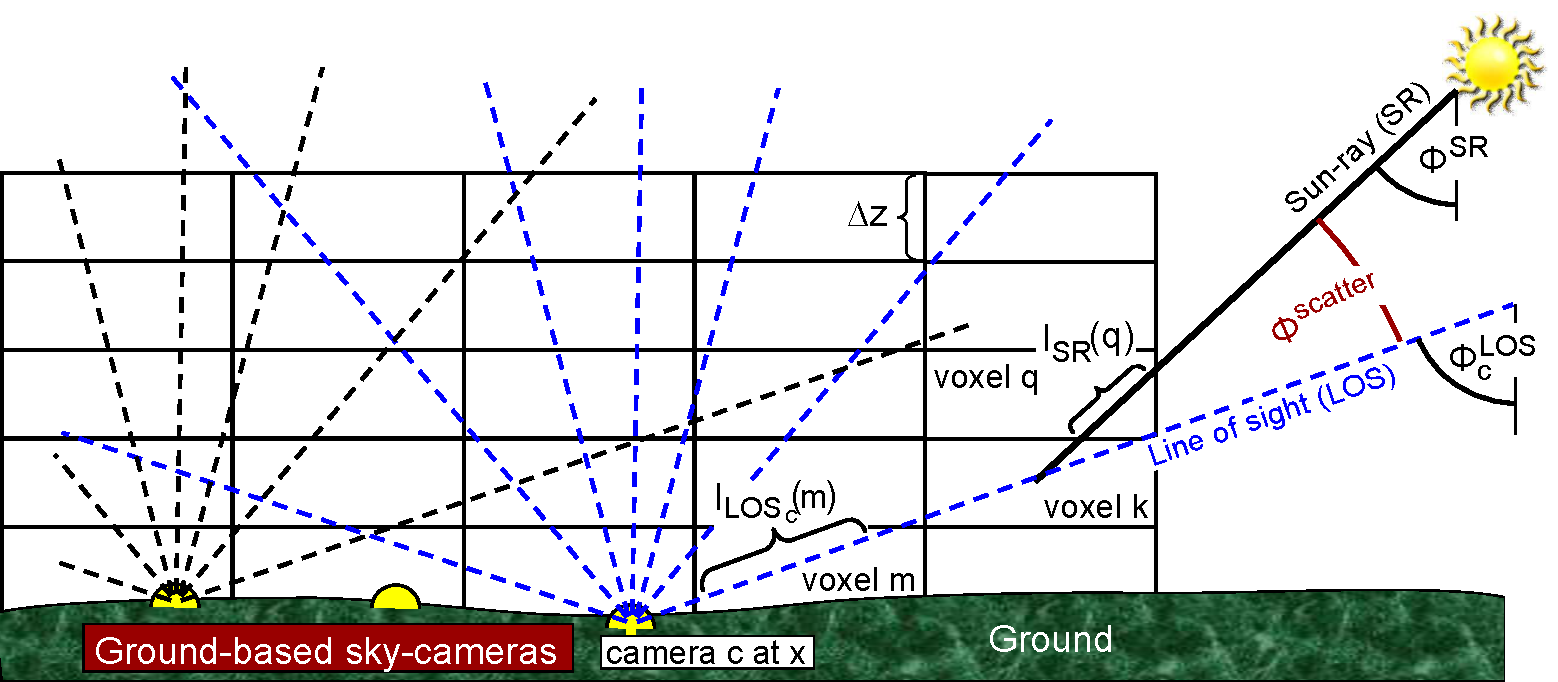
\includegraphics[width=\linewidth]{images/groundtomog24.pdf}}
  \end{center}
  \caption{\small Lightfield imaging through a volumetric distribution
    in the atmosphere, using ground-based cameras.}
  \label{fig:groundgrid}
\end{figure*}
Projecting this large object to various directions is similar to
tomography in other scientific domains. However, the formulation here
is distinct. Most tomography setups have a controlled and/or
multidirectional radiation source~\cite{gorbunov,messer}. In contrast,
our source is the uncontrolled, unidirectional Sun. Moreover, typical
tomography relies on a linear model~\cite{gregson}: the pixel value is
a linear combination of components along a line of sight (LOS), or a
multiplicative combination (linearized by a logarithm). Linear
tomography can detect volcanic gas~\cite{wright}, which absorbs
UV. Other gases in the atmosphere absorb IR. However, in visible
light, atmospheric attenuation is typically dominated by {\em
  scattering} by particles (aerosols), rather than absorption by
gasses. Thus, in our problem, we cannot rely on direct illumination,
but on sunlight scattered into the LOS.  The model turns out to be
{\em nonlinear, yet tractable}.

We do not deal with clouds here. Clouds scatter sunlight very strongly
and are easily observed. Hence they are directly recovered using
common stereoscopic tools, similarly to opaque surfaces~\cite{seiz}.
On the other hand, aerosols have much more subtle visual effects and
are thus more difficult to recover. We focus on them.  In remote
sensing~\cite{diner}, imaging through air is associated with {\em
  atmospheric correction}, based on {\em aerosol retrieval}. In this
discipline, the atmosphere is often assumed to be plane-parallel, for
simplicity, using only 1D vertical RT. Consequently
state-of-the-art aerosol retrieval is done in distinct large lateral
blocks~\cite{Martonchikc} with limited height
resolution~\cite{kalashnikova}. We, however, seek high resolution 3D
recovery. Computational photography offers new ways to peer into
media. In addition to active descattering~\cite{fuchs,kim,Ng1948} and
recovery of refractive transparent objects~\cite{ihrke}, overcoming
the atmosphere~\cite{Joshi2010,Zhu2013} to view ground objects was
studied in horizontal, fixed
views~\cite{fattal,he,Chen,kratz,narasimhan2,oakley,Hschechner2,tan}. In
this paper, however, the medium itself, at all relevant altitudes is
the object of interest.

3D recovery of this medium has direct implications to various
scientific communities that either rely on remotely-sensed imagery,
study the atmosphere, or overcome the medium to see beyond. These
include meteorology, atmospheric sciences, volcanology, and
climatology.  Aerosol retrieval is important for understanding climate
evolution~\cite{Dayan2008,kalashnikova} and monitoring air
quality. Mapping aerosol density is significant to aviation safety,
which needs real time assessment of conditions and visibility around
flight paths. To keep safe, today's coarse sensing limits flight
capacity. A prominent example is the 2010 eruption of Iceland's
Eyjafjallaj$\ddot {\rm o}$kull volcano, whose ash (aerosols) covered
much of Europe's airspace, grounding $\approx 100,000$
flights. Knowing the 3D distribution of aerosol density may indicate
safe 3D corridors to safely pass through, enhancing airspace
use. Viewing beyond the medium, atmospheric correction is needed, for
example, in satellite tracking of chlorophyll
distributions~\cite{johnsen}. Additional bodies in the solar system
have atmospheres. These objects can be viewed from multiple directions
by probes.  The approach described here may be helpful there.

We model passive optical tomographic imaging of 3D atmospheric
scatterer distributions in cloudless conditions. Then, we solve this
tomography problem, to recover the distribution. Recovery is
formulated as an optimization that minimizes a cost function. We
derive the gradient of this cost function, to enable efficient
optimization.

%%%%%%%%%%%%%%%%%%%%%%%%%%%%%%%%%%%%%%%%%%%%%%%%%%%%%%%%%%%%
%%%%%%%%%%%%%%%%%%%%%%%%%%%%%%%%%%%%%%%%%%%%%%%%%%%%%%%%%%%%

\section{Related Work}
\label{sec:literature}

{\em Lightfield}, or {\em integral}
imaging~\cite{Ng2006,bishop,Ng1948}, samples the radiance distribution
in location and direction. It has so far been used in small-scale
setups. Our proposed research deals with huge scale, up to Earth's
size. Capturing the lightfield in very large scales requires uncommon
sensors. Sampling Earth both spatially and angularly is done by the
Multiangle Imaging SpectroRadiometer (MISR)~\cite{Martonchikc} from
space, the Airborne Multiangle SpectroPolarimetric
Imager (AirMSPI)~\cite{dinerDavis10}, and other spaceborne and
airborne instruments.

Dehazing strives to improve quality of images taken through a
semi-transparent medium, be it murky liquid~\cite{kim,fuchs},
haze~\cite{fattal,Hschechner2}, or fog~\cite{narasimhan2}.  In remote
sensing~\cite{kokhan}, imaging through air is associated with {\em
  atmospheric correction}, based on {\em aerosol retrieval}.  In this
methods the medium is usually assumed to be uniform or at least
plane-parallel.  We, however, seek 3D recovery.  Another major
difference is that these methods see the translucent medium as a
disturbance that algorithms need to overcome, while in our research it
is the medium that we want to recover.

Computed Tomography (CT) refers to the reconstruction of a 3D object
from a collection of projections of the object using any kind of
penetrating radiation. CT finds wide use in medical imaging but is
also valuable in other scientific fields, like
geophysics~\cite{Kazahaya2008}, material science~\cite{Baruchel2000},
astrophysics, and more.  Imaging of gaseous materials is also the
target of extensive CT research~\cite{Price2001,Cosofret2009}. CT is
based on an image formation model that describes the physical process
underlying the projected measurements.  Most image formation models
assume either absorption or emission processes. Other image formation
models assume dominant diffusion by scattering~\cite{Boas2001}.

CT uses several different methods for reconstructing the underlying
medium. Transform algorithms are based on the Fourier and Radon
transforms. Both relate the projection (or its Fourier transform) to
the medium (or its Fourier transform). Solving for the medium involves
calculating the inverse transform in an iterative process.  These
algorithms assume a linear image formation model and require large
amount of projections to give reasonable results. The simultaneous
algebraic reconstruction technique
(SART)~\cite{KakAvinashC.andSlaney2001} is another common method which
is used when the image formation model is too big for explicit matrix
representation. Stochastic Tomography~\cite{gregson} uses a different
approach where the reconstruction is done in the space of projections
using a probabilistic process based on random walk. This bypasses the
need to discretize the signal, usually represented over a grid, and
the use of large matrices to represent the formation model.

Our research topic is closely related to optical
tomography~\cite{Arridge}. Optical tomography uses light to visualize
tissue, usually from close range.  Due to the highly scattering nature
of biological tissue, optical tomography uses diffusive approximation
in the image formation model.  Another method, based on scattering, is
the X-Ray Scatter CT~\cite{Aviles2011} which measures the absorption
and scattering coefficients of the medium separately.
 
However, the formulation of our problem is {\em different} than prior
situations. Most tomography setups have a controlled and/or
multidirectional radiation source~\cite{messer}. In contrast, our
source is the uncontrolled, unidirectional Sun. Moreover, typical
tomography relies on a linear model: the pixel value is a linear
combination of components along a line of sight (LOS), or a
multiplicative combination which is linearized by a logarithm.
However, photographs of the atmosphere are a mixture of {\em
  scattering}, and absorption. The model turns out to be {\em
  nonlinear, yet tractable}.

%%%%%%%%%%%%%%%%%%%%%%%%%%%%%%%%%%%%%%%%%%%%%%%%%%%%%%%%%%%%
%%%%%%%%%%%%%%%%%%%%%%%%%%%%%%%%%%%%%%%%%%%%%%%%%%%%%%%%%%%%

\section{Theoretical Background}
\label{sec:theor-backgr}

\noindent {\bf Extinction}: Sun rays (SR) irradiate a small volume
that includes particles of a certain type.  Each particle has an {\em
  extinction cross section} $\sigma$ (units \si{\meter\squared}) for
interacting with the irradiance. The density of the particles is $n$
(units \si[sticky-per]{\per\cubic\metre}). Per unit volume, the {\em
  extinction coefficient} $\beta$ is
\begin{align}
  \beta= \sigma n \;.
  \label{eq:extinctc}
\end{align}
The volume has infinitesimal length $dl$. Then, the relative portion
of extinct SR irradiance is the unitless differential {\em optical
  depth}
\begin{align}
  d\tau= \beta dl=\sigma n dl \;.
  \label{eq:extinct}
\end{align}
The optical depth aggregates in extended propagation:
\begin{align}
  \tau= \int d\tau=\int \beta dl=\int \sigma n dl \;.
  \label{eq:tau}
\end{align}
Through an attenuating volume, the {\em transmittance} exponentially
decays with the optical depth:
\begin{align}
  t=\exp(-\tau)
  \label{eq:beer-lambert}
\end{align}

\noindent {\bf Scattering}: Interaction of a single particle with the
irradiance is by absorption and scattering. The weight of scattering
(to all directions), relative to the total extinction is given by the
unitless {\em single scattering albedo} $\varpi$ of the particle. The
{\em scattering coefficient} $\alpha$ is
\begin{align}
  \alpha= \varpi\beta=\varpi \sigma n \;.
  \label{eq:alph}
\end{align}
The angular distribution of scattering is determined by a {\em phase
  function} $P$. Part of the light scatters towards a camera's LOS, as
illustrated in \cref{fig:groundgrid}. The angle between the SR and LOS
is the scattering angle $\Phi^{\rm scatter}$. The phase function
$P(\Phi^{\rm scatter})$ is normalized: its integral over all solid
angles is unit. The {\em angular scattering coefficient}
$\tilde\alpha$ (units \si[sticky-per]{\per\meter\steradian}) is
\begin{align}
  \tilde\alpha(\Phi^{\rm scatter}) = \varpi\beta P(\Phi^{\rm scatter})
  = \varpi \sigma n P(\Phi^{\rm scatter}).
  \label{eq:alphabasic}
\end{align}

The phase function is often approximated by a parametric expression,
as the Henyey-Greenstein~\cite{Cornette1995} function,
\begin{align}
  P_g(\Phi^{\rm scatter})\approx \sfrac{3}{8\pi} (1 - g^2)(1+\mu^2)
  (2+g^2)^{-1}(1 + g^2 - 2g\mu)^{\sfrac{-3}{2}}
  \label{eq:aerosol_scatter}
\end{align}
where $g$ is an {\em anisotropy parameter} and $\mu\equiv \cos \Phi^{\rm scatter}$.
\\

\noindent {\bf Air molecules}: Scattering by air molecules follows the
{\em Rayleigh} model:
\begin{align}
  P^{\rm air}\left[\mu(k)\right] &\approx \sfrac{3}{16\pi}(1+\mu^2)
  \label{eq:rayleighP}
\end{align}
and $\varpi^{\rm air}$=1. Air molecular density $n^{\rm air}$ falls
off approximately exponentially with altitude, with a
characteristic~\cite{Levi1980} falloff height $H^\mathrm{air}=8\
\si{\km}$. Consequently~\cite{Levi1980}, the coefficients for
extinction and scattering by air molecules can be modeled by
\begin{align}
  \alpha^{\rm air}(h, \lambda)=\beta^{\rm air}(h, \lambda) \approxeq
  1.09 \times 10^{-3}\lambda^{-4}
  \exp(-h/H^\mathrm{air}) %\left[-\frac{h}{H^\mathrm{air}}\right].
  \label{eq:rayleighbeta}
\end{align}

%%%%%%%%%%%%%%%%%%%%%%%%%%%%%%%%%%%%%%%%%%%%%%%%%%%%%%%%%%%%
%%%%%%%%%%%%%%%%%%%%%%%%%%%%%%%%%%%%%%%%%%%%%%%%%%%%%%%%%%%%

\section{Methodology}
\label{sec:methodology}

We believe that high resolution atmospheric recovery can be achieved
by a set of ground-based wide-angle~\cite{Cossairt2011,
  Peleg01omnistereo:panoramic, Koppal:2011:WMS:2191740.2192152}
sky-cameras, looking upward, performing integral imaging of the sky.
Consider \cref{fig:groundgrid}.  Ground-based wide-angle sky-cameras
capture the sky lightfield from below. Per viewpoint, the view azimuth
and elevation angles (relative to the zenith and north) are
encapsulated in the vector ${\bm{\Theta}}$.  A raw image is $i_{\bm
  c}({\bm{\Theta}})$: a camera's location ${\bm x}$ is fixed, while
any pixel in a frame represents an angle ${\bm{\Theta}}$.  The
measured radiance in all locations ${\bm x}$ and angles
${\bm{\Theta}}$ is the {\em lightfield} $I({\bm
  x},{\bm{\Theta}})$.This paper takes the first step, of formulating
this principle and demonstrating feasibility using realistic
simulations.  We simulate RT through the atmosphere using two
models. The first is based on Monte Carlo (MC) methods
(\cref{sec:monte-carlo-simul}) and models
Multiple-Scattering. Therefore it enables simulating realistic
scenarios.  The second model uses the Single-Scattering approximation
(\cref{sec:single-scatt-model}). It is less accurate than the MC model
but it enables stating an analytic solution to the RT in a closed
form. This closed form is beneficial to us as it enables us to invert
the model and thus recover the underlying atmosphere
(\cref{sec:inverse-problem}). To mimic realistic scenarios, we apply
the reconstruction algorithm on images simulated by the MC model.

%%%%%%%%%%%%%%%%%%%%%%%%%%%%%%%%%%%%%%%%%%%%%%%%%%%%%%%%%%%%
%%%%%%%%%%%%%%%%%%%%%%%%%%%%%%%%%%%%%%%%%%%%%%%%%%%%%%%%%%%%

\section{Single-Scattering Model}
\label{sec:single-scatt-model}

A forward model takes as input the aerosol distribution, and outputs
images as if captured at various viewpoints.  In a
\emph{single-scattering} model, any SR changes direction only once on
the way to the camera. This model is valid in atmospheres that are not
very dense: inside fog and clouds this model does not apply.  Under
single-scattering approximation, radiative transfer has three steps
(\cref{fig:groundgrid}):
\begin{inparaenum}[\hfill\bfseries a\upshape)]
\item \label{itm:first} Attenuation of a SR propagating from the top
  of the atmosphere (TOA) to voxel $k$.
\item \label{itm:second} Light scattering at voxel $k$, towards a
  camera.
\item \label{itm:third} Light attenuation on the LOS from voxel $k$ to
  the camera.
\end{inparaenum}
Steps \ref{itm:first} and \ref{itm:third} involve the optical depth
along the light path to and from voxel $k$, analyzed in
\cref{sec:optical-depth}.  Step \ref{itm:second} involves the
scattering coefficient at voxel $k$, described in
\cref{sec:scattering}.

%%%%%%%%%%%%%%%%%%%%%%%%%%%%%%%%%%%%%%%%%%%%%%%%%%%%%%%%%%%%

\subsection{Optical Depth}
\label{sec:optical-depth}

An infinitesimal volume contains aerosols. The extinction and
scattering coefficients due to aerosols in this volume are,
respectively
\begin{equation}
  \beta^{\rm aerosol}=\sigma^{\rm aerosol} n^{\rm aerosol}
  \;\;,\;\;
  \alpha^{\rm aerosol}=\varpi^{\rm aerosol} \beta^{\rm aerosol}
  \;.
  \label{eq:betaer}
\end{equation}
The infinitesimal volume contain also air molecules. Hence, the
overall extinction and scattering coefficients in this small volume
are, respectively
\begin{equation}
  \beta=\beta^{\rm air}+\beta^{\rm aerosol}
  \;\;,\;\;
  \alpha=\alpha^{\rm air}+\alpha^{\rm aerosol}
  \;.
  \label{eq:betair}
\end{equation}

Any voxel generally contains both air molecules and aerosols. Voxels
are indexed by $k$ or $q$. As approximation, assume that within any
voxel, the molecular parameters $\{ \beta^{\rm air}(k),\alpha^{\rm
  air}(k)\}$ and the aerosol parameters $\{ \sigma^{\rm
  aerosol}(k),\varpi^{\rm aerosol}(k), n^{\rm aerosol}(k),g(k)\}$ are
constants, e.g., corresponding to the value at each voxel
center. These parameters may change between voxels.

A voxel's vertical geometric thickness is $\Delta z$.  The Sun zenith
angle is $\Phi^{\rm SR}$. Denote a SR line segment between the TOA and
the center of voxel $k$ by $[{\rm SR},k]$. This SR intersects voxel
$q$. The geometric length of this intersection line segment is $l_{\rm
  SR}(q)$ which depends on $\Delta z$, $\Phi^{\rm SR}$ and $q$.
Following \cref{eq:tau,eq:betair}, the optical depth between the TOA
and voxel $k$ is
\begin{equation}
  \tau_{\rm SR}(k)= \sum_{q \in[{\rm SR},k]} \beta(q) l_{\rm SR}(q) \;\;.
  \label{eq:lSRn}
\end{equation}
Based on \cref{eq:betaer,eq:betair,eq:lSRn},
\begin{equation}
  \tau_{\rm SR}(k)=
  \tau_{\rm SR}^{\rm air}(k) +  \tau_{\rm SR}^{\rm aerosol}(k)
  \;\;,
  \label{eq:lSRaa}
\end{equation}
where
\begin{equation}
  \tau_{\rm SR}^{\rm air}(k)=
  \sum_{q \in[{\rm SR},k]}
  \beta^{\rm air}(q)  l_{\rm SR}(q)
  \label{eq:lSRair}
\end{equation}
and
\begin{equation}
  \tau_{\rm SR}^{\rm aerosol}(k)
  \sum_{q \in[{\rm SR},k]}
  \sigma^{\rm aerosol}(q) n^{\rm aerosol}(q) l_{\rm SR}(q)
  \label{eq:lSRaeros}
\end{equation}

The number of voxels is $N_{\rm voxels}$. All their associated
variables are concatenated into columns stack vectors, each $N_{\rm
  voxels}$ long. Aerosol densities and cross sections in all voxels
are stored in the respective vectors ${\bm n}$ and
$\vect{\sigma}$. Define a $N_{\rm voxels}\times N_{\rm voxels}$ sparse
matrix ${\bm D}^{\mathrm{Sun \rightarrow voxel}}$, whose element
$(k,q)$ is
\begin{equation}
  D^{\mathrm{Sun \rightarrow voxel}}(k,q) =
  \left\{
    \begin{array}{ll}
      l_{\rm SR}(q) & \mbox{ if $q \in[{\rm SR},k]$} \\
      0  & \mbox{ otherwise}
      \label{eq:Dsv}
    \end{array}
  \right.
  .
  \hspace{-0.05cm}
\end{equation}
\cref{eq:lSRaeros,eq:Dsv} lead to a vector of SR optical depths due to
aerosols (See \cref{fig:projection})a:
\begin{equation}
  \vect{\tau}_{\rm SR}^{\rm aerosol}=
  {\bm D}^{\mathrm{Sun \rightarrow voxel}}
  (\vect{\sigma} \odot {\bm n})
  \label{eq:tauSRvec1}
\end{equation}
where the operator $\odot$ denotes the Hadamard (element-wise)
product. Similarly, \cref{eq:lSRair} leads to a vector of SR optical
depths due to air, $\vect{\tau}_{\rm SR}^{\rm air}$.

Analogously, for camera $c$, denote by $[{\rm LOS}_c,k]$ a LOS bounded
between the camera and the center of voxel $k$. The LOS zenith angle
is $\Phi^{\rm LOS}_c$.  This LOS intersects voxel $q$. The geometric
length of this intersection line segment is $l_{\rm LOS_c}(q)$which
depends on $\Delta z$, $\Phi^{{\rm LOS}_c}$ and $q$.  Analogously to
\cref{eq:lSRaa,eq:lSRair,eq:lSRaeros}, the optical depth along a LOS
to $k$ is
\begin{equation}
  \tau_{{\rm LOS}_c}(k)=
  \tau_{{\rm LOS}_c}^{\rm air}(k) +  \tau_{{\rm LOS}_c}^{\rm aerosol}(k)
  \;\;,
  \label{eq:lLOSaerot}
\end{equation}
where
\begin{equation}
  \tau_{{\rm LOS}_c}^{\rm air}(k)=
  \sum_{q \in[{\rm LOS}_c,k]}
  \beta^{\rm air}(q)  l_{\rm LOS_c}(q)
  \label{eq:lLOSair}
\end{equation}
and
\begin{align}
  \label{eq:lLOSaeros}
  \tau_{{\rm LOS}_c}^{\rm aerosol}(k) = \sum_{q \in[{\rm LOS}_c,k]}
  \sigma^{\rm aerosol}(q) n^{\rm aerosol}(q) l_{\rm LOS_c}(q).
\end{align}
\cref{eq:lLOSaeros} leads to a vector of LOS optical depths due to
aerosols:
\begin{equation}
  \vect{\tau}_{{\rm LOS}_c}^{\rm aerosol}=
  {\bm D}^{\mathrm{voxel \rightarrow cam}}_c
  (\vect{\sigma} \odot {\bm n})
  \label{eq:tauLOSvec1}
\end{equation}
Here ${\bm D}^{\mathrm{voxel \rightarrow cam}}_c$ is a $N_{\rm
  voxels}\times N_{\rm voxels}$ sparse matrix whose element $(k,q)$ is
\begin{equation}
  D^{\mathrm{voxel \rightarrow cam}}_c(k,q) =
  \left\{
    \begin{array}{ll}
      l_{\rm LOS_c}(q) & \mbox{ if $q \in[{\rm LOS}_c,k]$} \\
      0  & \mbox{ otherwise}
      \label{eq:Dvc}
    \end{array}
  \right.
  .
  \hspace{-0.05cm}
\end{equation}
Similarly, \cref{eq:lSRair} leads to a vector of LOS optical depths
due to air, $\vect{\tau}_{{\rm LOS}_c}^{\rm air}$.

The fixed sparse matrices ${\bm D}^{\mathrm{Sun \rightarrow voxel}}$
and ${\bm D}^{\mathrm{voxel \rightarrow cam}}_c$ are compounded to a
single matrix
\begin{equation}
  {\bm D}_c=
  {\bm D}^{\mathrm{Sun \rightarrow voxel}}+
  {\bm D}^{\mathrm{voxel \rightarrow cam}}_c
  \;\;.
  \label{eq:Dtotal}
\end{equation}
Similarly, the molecular optical depths along all trajectories between
the sun, each voxel and camera $c$ are compounded to a vector
\begin{equation}
  \vect{\tau}_c^{\rm air}=
  \vect{\tau}_{\rm SR}^{\rm air}+
  \vect{\tau}_{{\rm LOS}_c}^{\rm air}
  \;\;.
  \label{eq:tauairtotal}
\end{equation}
Using \cref{eq:rayleighbeta} for $\beta^{\rm air}$ in all voxels, the
vector $\vect{\tau}_c^{\rm air}$ is fixed. Thus $\vect{\tau}_c^{\rm
  air}$ can be calculated once, per sun zenith angle.

Using
\cref{eq:lSRaa,eq:tauSRvec1,eq:lLOSair,eq:tauLOSvec1,eq:Dtotal,eq:tauairtotal},
the total optical depths corresponding to LOSs (of camera $c$) and SRs
that cross all voxels comprise the vector
\begin{equation}
  \vect{\tau}_c= \vect{\tau}_c^{\rm air}
  + {\bm D}_c (\vect{\sigma} \odot {\bm n})
  \;\;.
  \label{eq:tautotal}
\end{equation}
This vector depends on the variables $\vect{\sigma}$ and ${\bm n}$
(See~\cref{fig:projection}a).

%%%%%%%%%%%%%%%%%%%%%%%%%%%%%%%%%%%%%%%%%%%%%%%%%%%%%%%%%%%%

\subsection{Scattering}
\label{sec:scattering}

Per camera $c$ and voxel $k$, the lines $[{\rm SR},k]$ and $[{\rm
  LOS}_c,k]$ intersect at a fixed angle $\Phi^{\rm scatter}_c(k)$,
which is pre-calculated.  Column-stacking all voxels yields the vector
representation of all scattering angles in the domain,
$\vect{\Phi}^{\rm scatter}_c$ per camera $c$. Similarly, the
single-scattering albdeos $\varpi^{\rm aerosol}$ in all voxels are
stacked to vector $\vect{\varpi}$.  Using
\cref{eq:alphabasic,eq:rayleighP,eq:betaer,eq:betair}, the angular
scattering coefficients across the domain are expressed in vector form
by
\begin{align}
  \tilde{\vect{\alpha}}^{\rm air}_c &=
  \vect{\beta}^{\rm air} \odot P^{\rm air}(\vect{\Phi}^{\rm scatter}_c) \nonumber \\
  \tilde{\vect{\alpha}}^{\rm aerosol}_c &= \vect{\varpi}\odot
  \vect{\sigma} \odot {\bm n} \odot P^{\rm aerosol}_{\bm
    g}(\vect{\Phi}^{\rm scatter}_c)
  \label{eq:alpha_matrix}
\end{align}
The vector ${\bm g}$ column-stacks the anisotropy parameter of the
phase function, in all voxels. We use this notation, to indicate a
parametric phase function as in \cref{eq:aerosol_scatter}.


%%%%%%%%%%%%%%%%%%%%%%%%%%%%%%%%%%%%%%%%%%%%%%%%%%%%%%%%%%%%

\subsection{Image Capture}
\label{sec:captured-image}

Compounding the attenuation of irradiance along both $[{\rm SR},k]$
and $[{\rm LOS}_c,k]$, and scattering by voxel $k$ towards the camera
(\cref{eq:beer-lambert,eq:betair,eq:tautotal}) the radiant power
contributed by the voxel is
\begin{equation}
  p_c(k)= L^{\rm TOA}
  [\tilde{\alpha}^{\rm air}_c(k) + \tilde{\alpha}^{\rm aerosol}_c(k)]
  e^{-\tau_c(k)}
  \;\;,
  \label{eq:ick}
\end{equation}
where $L^{\rm TOA}$ is the radiance at the TOA. A column-stack vector
of all voxel contributions is
\begin{equation}
  {\bm p}_c= L^{\rm TOA}
  [\tilde{\vect{\alpha}}^{\rm air}_c + \tilde{\vect{\alpha}}^{\rm aerosol}_c]
  \odot e^{-\vect{\tau}_c}
  \;\;.
  \label{eq:pc}
\end{equation}

A camera pixel collects light from a narrow cone in the
atmosphere. The cone includes some voxels, intersects with some other
voxels, and oblivious to all the rest~(\cref{fig:projection}b).
\begin{figure}
  \centering
  \yoavcomment{\def\svgwidth{0.8\columnwidth}\input{images/light_transfer.pdf_tex}}
  \caption{\small [a] Irradiance of voxel $k$ is attenuated by voxels
    above it on a SR. The scattered radiance from voxel $k$ is then
    attenuated by voxels below it on a LOS to camera $c$.  [b] An
    image pixel captures light emanating in a cone in space. Voxels
    that fully or partially fall in this cone are sensed by the
    pixel.}
  \label{fig:projection}
\end{figure}
Thus light power captured at a pixel is a weighted sum of the power
$p_c(k)$ from all voxels.  This linear sum is formulated by a matrix
operation over ${\bm p}_c$. The measured image is column-stacked to a
vector $N_{\rm pix}$ long. It is given by
\begin{equation}
  {\bm i}_c= {\vect{\Pi}}_c{\bm p}_c
  \;\;.
  \label{eq:IcP}
\end{equation}

Combining \cref{eq:tautotal,eq:pc,eq:IcP}, the captured image is thus
\begin{align}
  {\bm i}_c= L^{\rm TOA} {\vect{\Pi}}_c \left\{
    (\tilde{\vect{\alpha}}^{\rm air}_c + \tilde{\vect{\alpha}}^{\rm
      aerosol}_c) \odot e^{-[\vect{\tau}_c^{\rm air} + {\bm D}_c
      (\vect{\sigma} \odot {\bm n})]} \right\}
  \label{eq:bigIc}
\end{align}

To simplify the case in study, let us assume there is only a single
type of aerosol over a scene. Hence, the three-element vector
$[{\sigma}^{\rm aerosol},\varpi^{\rm aerosol},g]$ is uniform across
the scene, but the density distribution ${\bm n}$ is variable. Then,
\cref{eq:bigIc} degenerates to
\begin{align}
  {\bm i}_c= L^{\rm TOA} {\vect{\Pi}}_c \Big\{ e^{-(\vect{\tau}_c^{\rm
      air} + {\sigma}^{\rm aerosol} {\bm D}_c {\bm n}) }\odot
  [\tilde{\vect{\alpha}}^{\rm air}_c + \varpi^{\rm aerosol}\sigma^{\rm
    aerosol} P^{\rm aerosol}_g(\vect{\Phi}^{\rm scatter}_c) \odot{\bm
    n} ] \Big\} .
  \label{eq:bigIA}
\end{align}

%%%%%%%%%%%%%%%%%%%%%%%%%%%%%%%%%%%%%%%%%%%%%%%%%%%%%%%%%%%%
%%%%%%%%%%%%%%%%%%%%%%%%%%%%%%%%%%%%%%%%%%%%%%%%%%%%%%%%%%%%

\section{Inverse Problem}
\label{sec:inverse-problem}

%%%%%%%%%%%%%%%%%%%%%%%%%%%%%%%%%%%%%%%%%%%%%%%%%%%%%%%%%%%%

\subsection{Unknowns and Prior Knowledge}
\label{sec:prior}

In general terms, the variables are the set
\begin{equation}
  {\cal V}\equiv
  \left\{
    {\bm n},
    \left\{
      \vect{\varpi}_{\lambda},\vect{\sigma}_{\lambda},{\bm g}_{\lambda}
    \right\}_{\lambda}
  \right\}
  \;\;,
  \label{eq:calV}
\end{equation}
where $\lambda$ denotes the spectral (color) channel.  There are
$N_{\rm spectral}$ spectral channels.  Thus, the number of unknown
variables is in principle \mbox{$|{\cal V}|=N_{\rm voxels}(1+3N_{\rm
    spectral})$}.

Prior knowledge reduces the unknowns. For simplicity we assume a
single aerosol type dominates a scene. Furthermore, in the following
section we assume that we know the type of the particle. Hence, we
focus here on retrieving ${\bm n}$.

%%%%%%%%%%%%%%%%%%%%%%%%%%%%%%%%%%%%%%%%%%%%%%%%%%%%%%%%%%%%

\subsection{Objective Function}
\label{sec:objective-function}

The recovery task is phrased as optimization of an objective function,
that fits the image-formation model (\cref{eq:bigIc,eq:bigIA}) to
measured photographs $\{ {\bm i}^{\rm measured}_c\}_{c=1}^{N_{\rm
    views}}$:
\begin{equation}
  \label{eq:minobjectiveA}
  \hat{\bm n} =
  \argmin_{{\bm n}} F({\bm n})
\end{equation}
where
\begin{equation}
  \label{eq:objectiveA}
  F({\bm n})
  = \sum_{c=1}^{N_{\rm views}}
  \| \Mask \roundy{{\bm i}^{\rm measured}_c - {\bm i}_c({\bm n})}\|^2_2 + \eta \cdot \Psi({\bm n})
\end{equation}
Here $\Psi({\bm n})$ is a regularization term that expresses some
prior knowledge on the solution and $\eta$ is the regularization
coefficient.  We enforce smoothness of the solution by using the
\emph{Laplacian} operator.
\begin{equation}
  \label{eq:regularizer}
  \Psi({\bm n}) = \| \nabla^2{\bm n}\|^2_2
\end{equation}
We use $\Mask$ as a weight map to mask the influence of the sun and
the horizon. These regions are prone to dominant multiple scattering.
We solve~\cref{eq:minobjectiveA} using standard optimization tools.
The gradient of $F$ with respect to ${\bm n}$ is
\begin{align}
  \Grad{{\bm n}} F = -2\sum_{c=1}^{N_{\rm views}}
  \transpose{\left[{\bm J}_{{\bm i}_c}({\bm n})\right]} [{\bm i}^{\rm
    measured}_c - {\bm i}_c({\bm n})] + 2 \cdot \eta \cdot
  \nabla^2\nabla^2{\bm n} \;.
  \label{eq:gradient1}
\end{align}
Here the matrix ${\bm J}_{{\bm i}_c}({\bm n})$ is the Jacobian of the
vector ${\bm i}_c$ with respect to ${\bm n}$, and we make use of the
symmetry of the \emph{Laplacian} operator. A close-form expression of
our Jacobian is
\begin{align}
  {\bm J}_{{\bm i}_c}({\bm n}) &= L^{\rm TOA}({\bm A}-{\bm B}){\bm C}
  ,
  \label{eq:gradient2}
\end{align}
where
\begin{align}
  \label{eq:gradient3}
  {\bm A} &= \varpi^{\rm aerosol}\sigma^{\rm aerosol}
  \OpDiag{ P_g^{\rm aerosol}(\vect{\Phi}^{\rm scatter}_c)} \nonumber\\
  {\bm B} &= {\sigma}^{\rm aerosol}\transpose{{\bm D}_c} \nonumber\\
  & \;\;\; \OpDiag{[\tilde{\vect{\alpha}}^{\rm air}_c + \varpi^{\rm
      aerosol}\sigma^{\rm aerosol} P^{\rm aerosol}_g(\vect{\Phi}^{\rm
      scatter}_c) \odot{\bm n}
    ]} \nonumber \\
  {\bm C} &= \OpDiag{\exp[-(\vect{\tau}_c^{\rm air} + {\sigma}^{\rm
      aerosol} {\bm D}_c {\bm n})]} \transpose{{\vect{\Pi}}_c}
\end{align}
For a detailed derivation of \cref{eq:gradient2,eq:gradient3}, we
refer the reader to \cref{sec:gradient-derivation}.

%%%%%%%%%%%%%%%%%%%%%%%%%%%%%%%%%%%%%%%%%%%%%%%%%%%%%%%%%%%%
%%%%%%%%%%%%%%%%%%%%%%%%%%%%%%%%%%%%%%%%%%%%%%%%%%%%%%%%%%%%

\section{Monte Carlo RT}
\label{sec:monte-carlo-simul}

Monte Carlo (MC) methods enable rigorous modeling of photon
propagation in the atmosphere. The radiative transfer is expressed as
probability distributions which describe the distance travelled by the
photon between scatterings and the angle of deflection at each
scatter.  This enables simulating multiple scattering and produce
realistic results.  MC simulations can be made arbitrarily accurate by
increasing the number of photons.  Another advantage of the MC methods
is that they are highly parallelizable.

The MC simulations use the same atmosphere grid described in
\cref{sec:single-scatt-model}. we use backward MC, i.e. photons are
traced from the detector to the sun. Photons are emitted from each
pixel of the camera in the direction determined by the camera
model. The optical distance that the photon travels before scattering
is determined according to the Beer-Lambert law~\cref{eq:beer-lambert}
and the inversion sampling method. Once the optical distance is
determined the ``real'' distance is determined by summing the optical
depth of the discrete voxels (\cref{sec:optical-depth}) along the
photon direction till the desired optical distance is reached.  At
each scattering event, first the type of aerosol is determined by
sampling the different aerosols distributions inside the voxel. The
new direction is determined by inverse sampling the phase function of
the relevant aerosols: Rayleigh, \cref{eq:rayleighP} or
Henyey-Greenstein \cref{eq:aerosol_scatter}.  To accelerate the MC we
use the local estimation (LE) method.


%%%%%%%%%%%%%%%%%%%%%%%%%%%%%%%%%%%%%%%%%%%%%%%%%%%%%%%%%%%%
%%%%%%%%%%%%%%%%%%%%%%%%%%%%%%%%%%%%%%%%%%%%%%%%%%%%%%%%%%%%

\section{Simulations}
\label{sec:simul}

To test the model, we made simulations based on atmospheric models in
the literature. Here are the details.

\noindent{\bf Sun}: The sun is at zenith angle $\Phi^{\rm
  SR}=45^o$. Its $L^{\rm TOA}$ is obtained
from~\cite{BBradiance,sun_composition}, with respective red-green-blue
ratios of $L^{\rm TOA}_{\rm R}:L^{\rm TOA}_{\rm G}:L^{\rm TOA}_{\rm
  B}=255:236:224$.

\noindent{\bf Dimensions}: The domain of sky we simulate and recover
has area of \SI{50 x 50}{\km}, and it extends from the ground up to
altitude of \SI{10}{\km}. This volume is divided into a rectilinear
grid. We used different grid sizes from \num{50 x 50 x 100} grid,
where each voxel has area of \SI{1 x 1}{\km} and vertical thickness of
\SI{100}{\metre} and down to num{10 x 10 x 20} grid, where each voxel
has area of \SI{5 x 5}{\km} and vertical thickness of
\SI{500}{\metre}. The different grid sizes determine the number of
variables.

\noindent{\bf Aerosol}: We used particle-type 6 from the aerosol list
in Ref.~\cite{Martonchik2009}. This is a spherical non-absorbing
sea-salt/organic particle, whose anisotropy parameter per color
channel is $[g_{\rm R},g_{\rm G},g_{\rm B}]=[0.763,0.775,0.786]$. Its
corresponding extinction cross sections are $[\sigma^{\rm
  aerosol}_{\rm R}, \sigma^{\rm aerosol}_{\rm G}, \sigma^{\rm
  aerosol}_{\rm
  B}]=[16.5,16.2,15.9]$~\si[sticky-per]{\per\micro\meter\squared}.
Its single-scattering albedo is $\varpi^{\rm aerosol}=1$ at all
channels.

We simulated various spatial distributions. All were set as a product
of two functions. The first function is an exponential
decay~\cite{Levi1980} with altitude $h(k)$ of voxel $k$,
\begin{align}
  w_1[h(k)] = \frac{1} {n^{sea level}}
  \exp\left[-\frac{h(k)}{H^\mathrm{aerosol}}\right],
\end{align}
where $H^\mathrm{aerosol}=2$~\si{\km}. This expresses a general trend
of reduced atmospheric density with height.

The second function, $w_2$, expresses a clustered nature of aerosol
``clouds''. We define blobs in the form of 3D ellipsoids. There may be
multiple ellipsoids suspended.  Then
\begin{equation}
  w_2(k) =
  \left\{
    \begin{array}{ll}
      1  & \mbox{ if $k\in$ any blob cluster} \\
      0  & \mbox{ otherwise}
      \label{eq:f2}
    \end{array}
  \right.
  .
  \hspace{-0.05cm}
\end{equation}
The true aerosol distribution is then
\begin{equation}
  \label{eq:ntrue}
  {\bm n}^{\rm true}={\bm w}_1\odot {\bm w}_2  .
  \hspace{-0.05cm}
\end{equation}
As an example, we created a {\em Haze Blobs} scene using two ellipsoid
blobs (\cref{fig:two_clouds_sim}a): the first is centered at altitude
\SI{3.3}{\km}, and has horizontal width of \SI{32}{\km} and vertical
thickness of \SI{2.8}{\km}. The second ellipsoid is centered at
altitude \SI{6.6}{\km}, and has lateral width of \SI{24}{\km} and
vertical thickness of \SI{2.1}{\km}. Note that the horizontal widths
are much larger than the vertical ones. This is consistent with scales
of atmospheric aerosol distributions.

\noindent{\bf Cameras}: The cameras are created by the MC simulations.
Each ground-based camera has a hemispherical field of view, capturing
the entire sky from its viewpoint. Again, we used different numbers of
cameras ranging from 100 viewpoints to 12. The cameras are arranged on
a grid.  The resolution of each camera is low, expressing the fact
that cloudless (yet hazy) sky images are rather smooth, hence there is
no need for high image resolution.  For example,
\cref{fig:simulation-results1}b shows an example of a modeled
photograph
\begin{figure}
  \centering
  \yoavcomment{\def\svgwidth{0.95\columnwidth}\input{images/ref_images.pdf_tex}}
  \caption{\small [a] Photograph of a sky that includes {\em Haze
      Blobs} rendered using the single-scattering model.  A yellow dot
    marks the Sun location. Dashed white circles mark elevation
    angles.  [b] Photograph of the same sky and view point rendered
    using the MCRT simulation (\cref{sec:monte-carlo-simul}).
    [c] Cross section along the 
  }
  \label{fig:simulation-results1}
\end{figure}
of the {\em Haze Blobs} scene that corresponds to
\cref{fig:two_clouds_sim}a.

\noindent{\bf Computer}: We had access to an SGI-TNN cluster computer
that has 88 computer nodes consisting of two 2.40 GHz six-Core Xeon
with 8GB DDR3 memory per core. The number of cures used is depends on
the size of the simulations. Each core was dedicated to rendering a
modeled image.

\noindent{\bf Optimization}: We used the L-BFGS-B
algorithm~\cite{BFGS}. The algorithm was initialized by ${\bm
  n}=0$. Satisfactory convergence occurred in several thousand
iterations, taking a couple of hours to complete in total.

%%%%%%%%%%%%%%%%%%%%%%%%%%%%%%%%%%%%%%%%%%%%%%%%%%%%%%%%%%%%
%%%%%%%%%%%%%%%%%%%%%%%%%%%%%%%%%%%%%%%%%%%%%%%%%%%%%%%%%%%%

\section{Results}
\label{sec:optimization-results}

An iso-surface visualization of the original {\em Haze Blobs}
distribution is shown in \cref{fig:two_clouds_sim}a, while the
recovered 3D distribution is visualized in
\cref{fig:two_clouds_sim}b. The distributions appear consistent,
though there are errors that stem from the random noise in the
images. To quantify the results, we use a relative error measure based
on the $\ell_1$ norm
\begin{equation}
  \label{eq:ndiff}
  \epsilon=\frac{\| \hat{\bm n}  - {\bm n}^{\rm true} \|_1}
  {\| {\bm n}^{\rm true} \|_1} ,
\end{equation}
It is equivalent to the aerosol mass that is over and under-estimated
in all voxels, relative to the total aerosol mass in the scene.  In
the {\em Haze Blobs} case, $\epsilon=0.202$.

We created a {\em Haze Front} scene. \cref{fig:front_sim}a shows an
iso-surface visualization of this distribution.
\begin{figure}
  \centering
  \yoavcomment{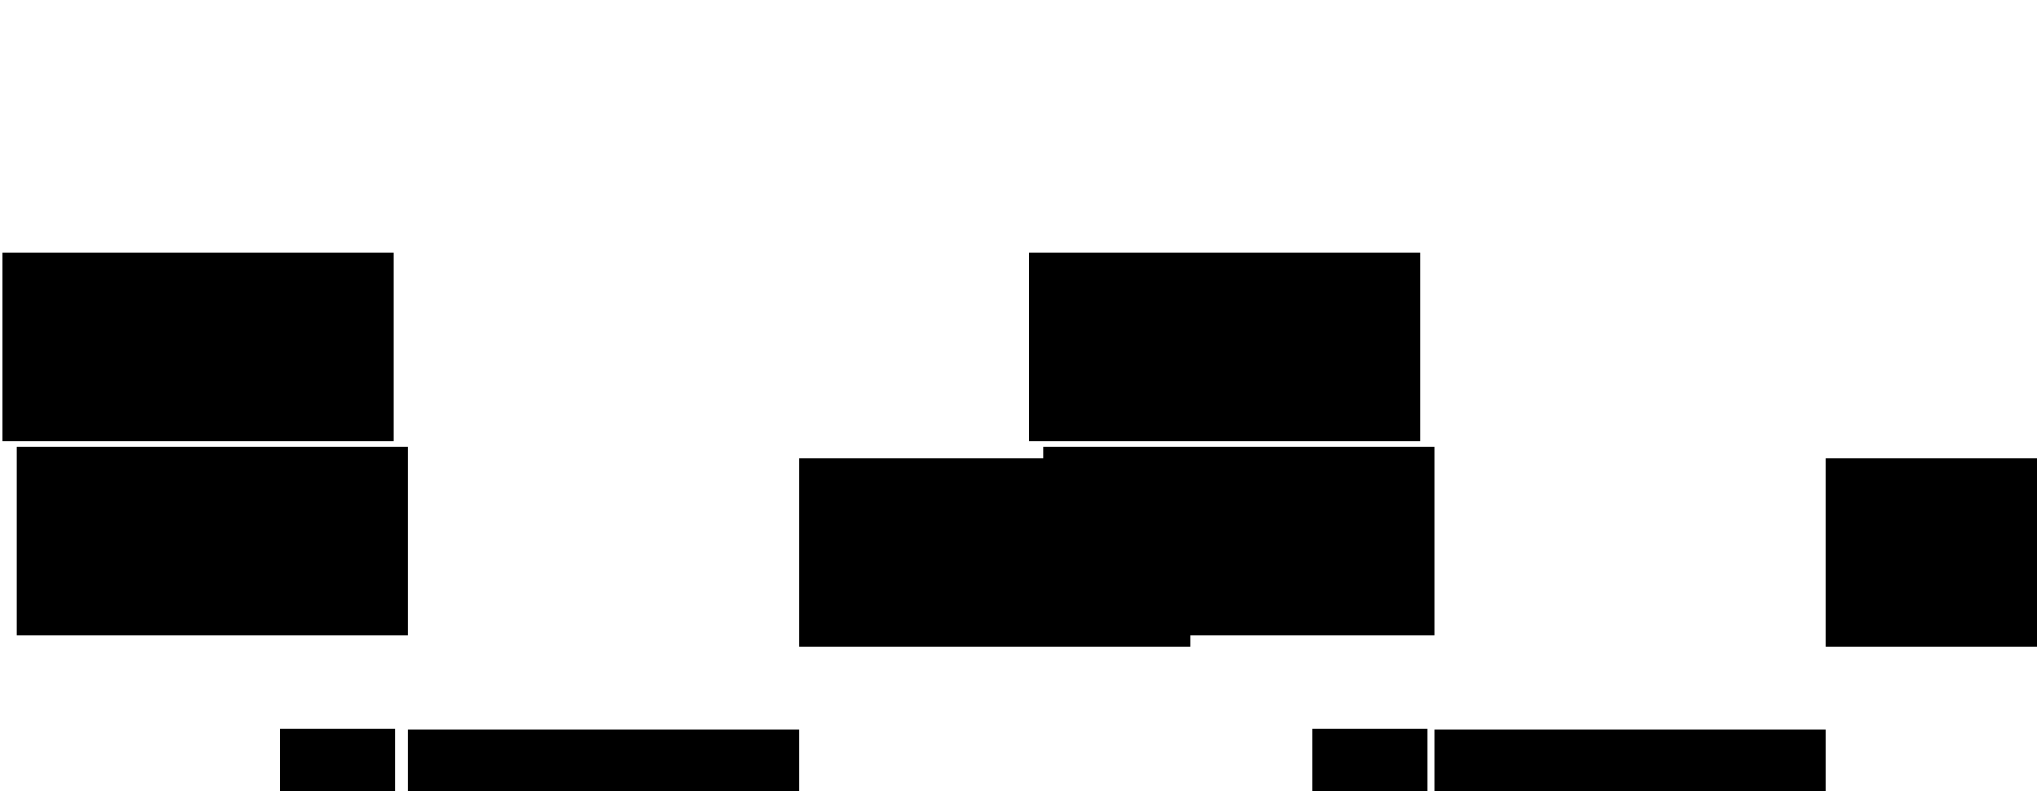
\includegraphics[width=\columnwidth]{images/two_clouds}}
  \caption{\small [a] Simulated 3D aerosol distribution composed of
    {\em Haze Blobs} and [b] its reconstruction. Color represents
    aerosol density. The density units are $10^{6}~{\rm
      particles}/{\rm m}^3.$}
  \label{fig:two_clouds_sim}
\end{figure}
\begin{figure}
  \centering
  \yoavcomment{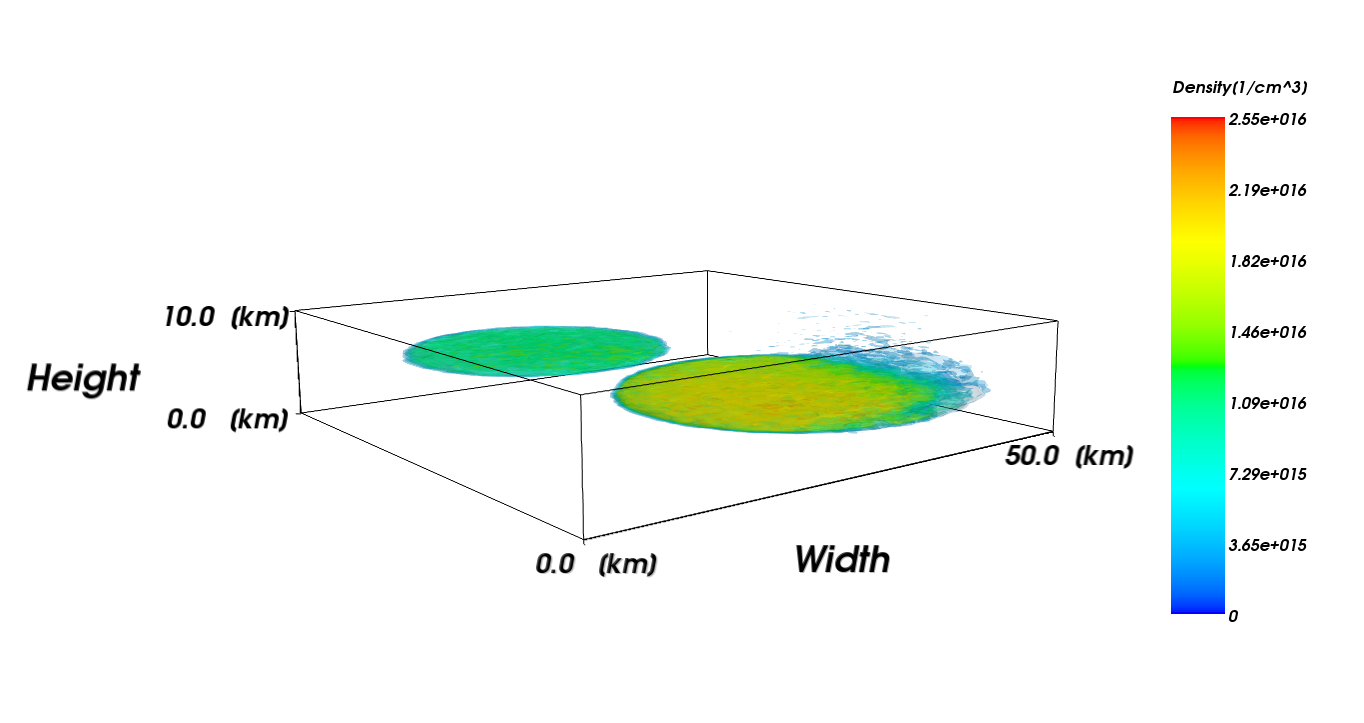
\includegraphics[width=\columnwidth]{images/front}}
  \caption{\small [a] Simulated 3D aerosol distribution composed of a
    {\em Haze Front}. [b] Its reconstruction. Color represents aerosol
    density. The density units are $10^{6}~{\rm particles}/{\rm
      m}^3.$}
  \label{fig:front_sim}
\end{figure}
Here an ellipsoid degenerated to an elliptic cylinder that partly
enters the analyzed volume. It is centered at altitude \SI{5}{\km},
has vertical thickness of \SI{4}{\km} and length of \SI{32}{\km} (only
part of which enters the volume). The haze front stretches across the
width of the volume.  \cref{fig:front_sim}b visualizes the recovered
3D distribution of this scene. For the {\em Haze Front},
$\epsilon=0.198$.

%%%%%%%%%%%%%%%%%%%%%%%%%%%%%%%%%%%%%%%%%%%%%%%%%%%%%%%%%%%%
%%%%%%%%%%%%%%%%%%%%%%%%%%%%%%%%%%%%%%%%%%%%%%%%%%%%%%%%%%%%

\section{Conclusions}
\label{sec:conclusions}

We describe a new way to sense the 3D atmosphere. We show feasibility
of departing from common 1D aerosol distribution models, in favor of
detailed 3D analysis.  The paper describes both a novel data
acquisition system concept for this recovery task, and a dedicated
algorithm for reconstructing aerosol distributions.

Even without regularization, the reconstruction algorithm handles
arbitrary density distributions. Using more prior knowledge,
e.g. spatial smoothness will improve the recovery.  The algorithm uses
a single scattering model. This approximation is valid when the
optical depth is small, which is common. To handle dense atmospheric
conditions (smoke, clouds), multi-scattering must be incorporated.

The goal, of coarse, is to deploy such a system on a very large
scale. However, this must first ensure that camera units are both cost
effective and field-robust, and that their positioning density is
proper. This will require a long-term engineering effort. Camera
specifications should be set to optimally recover a wide range of
aerosol distributions. This requires a major theoretic and numerical
research and development phase.  The new sensing modality and object
of interest offer a new domain for computational photography
problems. For example, how can compressed sensing principles be
employed here? How can priors be used to make data acquisition more
efficient? How can such a system be calibrated over time? Many such
questions and solutions would rise.


%%%%%%%%%%%%%%%%%%%%%%%%%%%%%%%%%%%%%%%%%%%%%%%%%%%%%%%%%%%%
%%%%%%%%%%%%%%%%%%%%%%% Appendix %%%%%%%%%%%%%%%%%%%%%%%%%
%%%%%%%%%%%%%%%%%%%%%%%%%%%%%%%%%%%%%%%%%%%%%%%%%%%%%%%%%%%%
\appendix

%%%%%%%%%%%%%%%%%%%%%%%%%%%%%%%%%%%%%%%%%%%%%%%%%%%%%%%%%%%%
%%%%%%%%%%%%%%%%%%%%%%%%%%%%%%%%%%%%%%%%%%%%%%%%%%%%%%%%%%%%

\section{Gradient Derivation}
\label{sec:gradient-derivation}

Here we detail the derivation of the gradient of the objective
function:
\begin{equation}
  \label{eq:objectiveA}
  F({\bm n})
  = \sum_{c=1}^{N_{\rm views}}
  \| {\bm i}^{\rm measured}_c - {\bm i}_c({\bm n})\|^2_2
\end{equation}
Here ${\bm i}^{\rm measured}_c$ is the image captured by camera $c$
and ${\bm i}_c({\bm n})$ is an image modeled from the viewpoint of
camera $c$ according to the density distribution ${\bm n}$. In
\cref{sec:captured-image} article we show that ${\bm i}_c({\bm n})$
can be expressed by
\begin{align}
  {\bm i}_c= L^{\rm TOA} {\vect{\Pi}}_c \Big\{ e^{-(\vect{\tau}_c^{\rm
      air} + {\sigma}^{\rm aerosol} {\bm D}_c {\bm n}) }\odot
  \;\;\;\;\;\;\;\;\;\;\;\;\;\;\;\;\;\;\;\;\;
  \nonumber \\
  [\tilde{\vect{\alpha}}^{\rm air}_c + %\right.
  \varpi^{\rm aerosol}\sigma^{\rm aerosol} P^{\rm
    aerosol}_g(\vect{\Phi}^{\rm scatter}_c) \odot{\bm n} ] \Big\} .
  \label{eq:bigIA}
\end{align}

The gradient of $F$ with respect to ${\bm n}$ is
\begin{align}
  \Grad{{\bm n}} F = -2\sum_{c=1}^{N_{\rm views}}
  \transpose{\left[{\bm J}_{{\bm i}_c}({\bm n})\right]} [{\bm i}^{\rm
    measured}_c - {\bm i}_c({\bm n})] \;.
  \label{eq:gradient1}
\end{align}
Here the matrix ${\bm J}_{{\bm i}_c}({\bm n})$ is the Jacobian of the
vector ${\bm i}_c$ with respect to ${\bm n}$. Element $(\Theta,k)$ of
this matrix differentiates the intensity in pixel ${\bm \Theta}$ (in
viewpoint $c$) with variation of the density at voxel $k$, i.e.,
$\partial i_c({\bm \Theta})/\partial{n^{\rm aerosol}(k)}$.

In order to describe the derivation of the Jacobian ${\bm J}_{{\bm
    i}_c}({\bm n})$, we first show some results relating to
differentiation. Let $\vect{n}$ be a vector of length $q$. Let
$\vect{g}(\vect{n})$ be a vector function: it outputs a vector of
length $r$. Let $\mat{B}$ be a $q \times r$ matrix and
\begin{align}
  \vect{g}(\vect{n}) = \exp^{-\transpose{\mat{B}}\vect{n}}.
  \label{eq:example1}
\end{align}
In \cref{eq:example1}, the exponential is element-wise (not raising an
operator to some power). Then
\begin{align}
  \label{eq:partial2}
  \PartDeriv{\vect{g}}{\vect{n}} &= - \mat{B} \,
  \OpDiag{\exp^{-\transpose{\mat{B}}\vect{n}}}
\end{align}
Here we denote by $\OpDiag{\vect{v}}$ conversion of vector $\vect{v}$
into a diagonal matrix, whose main diagonal elements correspond to the
elements of $\vect{v}$. Using \cref{eq:partial2} we can calculate
\begin{align}
  \label{eq:partial4}
  \PartDeriv{\exp^{-(\vect{\tau}_c^{\rm air} + {\sigma}^{\rm aerosol}
      {\bm D}_c {\bm n})}}
  {\vect{n}} &= - {\sigma}^{\rm aerosol}\transpose{\OpDistance_c} \,
  \OpDiag{\exp^{-(\vect{\tau}_c^{\rm air} + {\sigma}^{\rm aerosol}
      {\bm D}_c {\bm n})}}
\end{align}
In \cref{eq:partial4} we assume that $\vect{\tau}_c^{\rm air}$ is
known and constant.

To calculate the derivative of the Hadamard product in \cref{eq:bigIA}
we first note the following: Let $\vect{u}(\vect{n})$ be a vector
function that outputs a vector of length $r$. Let $\mat{B}$ be a $r
\times q$ matrix. Then,
\begin{align}
  \label{eq:partial1}
  \PartDeriv{\transpose{\mat{B}} (\vect{g} \odot \vect{u})}{\vect{n}}
  = \left[ \PartDeriv{\vect{g}}{\vect{n}} \OpDiag{\vect{u}} +
    \PartDeriv{\vect{u}}{\vect{n}} \OpDiag{\vect{g}} \right] \mat{B}.
\end{align}
Then,
\begin{align}
  \label{eq:partial3}
  \PartDeriv{\, \varpi^{\rm aerosol}\sigma^{\rm aerosol} P^{\rm
      aerosol}_g(\vect{\Phi}^{\rm scatter}_c) \odot{\bm n}}{\vect{n}}
  =
  \;\;\;\;\;\;\;\;\;\;\;\;\;\;\;\;\;\;\;\;\;\;\;\;\;\;\;\;\;\;\;\;\;\;\;\;\;\;\;\;\;\;
  \nonumber \\
  \varpi^{\rm aerosol}\sigma^{\rm aerosol}\OpDiag{P^{\rm
      aerosol}_g(\vect{\Phi}^{\rm scatter}_c)}
  \;\;\;\;\;\;\;\;\;\;\;\;\;\;\;\;\;\;\;\;
\end{align}

Based on \cref{eq:partial4,eq:partial1,eq:partial3} we can derive a
close-form expression for the Jacobian of \cref{eq:bigIA}:
\begin{align}
  {\bm J}_{{\bm i}_c}({\bm n}) &= L^{\rm TOA}({\bm A}-{\bm B}){\bm C}
  ,
  \label{eq:gradient2}
\end{align}
where
\begin{align}
  \label{eq:gradient3}
  {\bm A} &= \varpi^{\rm aerosol}\sigma^{\rm aerosol}
  \OpDiag{ P_g^{\rm aerosol}(\vect{\Phi}^{\rm scatter}_c)} \nonumber\\
  {\bm B} &= {\sigma}^{\rm aerosol}\transpose{{\bm D}_c} \nonumber\\
  & \;\;\; \OpDiag{[\tilde{\vect{\alpha}}^{\rm air}_c + \varpi^{\rm
      aerosol}\sigma^{\rm aerosol} P^{\rm aerosol}_g(\vect{\Phi}^{\rm
      scatter}_c) \odot{\bm n}
    ]} \nonumber \\
  {\bm C} &= \OpDiag{\exp[-(\vect{\tau}_c^{\rm air} + {\sigma}^{\rm
      aerosol} {\bm D}_c {\bm n})]} \transpose{{\vect{\Pi}}_c}
\end{align}


\end{document}

